\title{\textbf{ASVD: Activation-Aware Singular Value Decomposition for Attention Compression}}

\author{Anonymous authors}



\section{Introduction}

\subsection{Motivation}

The dominant storage cost in transformer models lies in the weight matrices 
of linear layers. For DistilBERT-base, the four attention projections 
($W_Q, W_K, W_V, W_O$) account for approximately 4.7 million parameters 
out of 66.9 million total (7\%). For RoBERTa-base, they account for 
9.4 million out of 124.6 million (7.5\%). Reducing these is the primary 
lever for model compression.

\textbf{Low-rank factorization} replaces each $W \in \mathbb{R}^{d_\text{out} \times d_\text{in}}$ 
with the product $U \Sigma V^\top$ where $U \in \mathbb{R}^{d_\text{out} \times r}$, 
$\Sigma \in \mathbb{R}^r$, and $V \in \mathbb{R}^{r \times d_\text{in}}$ for 
$r \ll \min(d_\text{in}, d_\text{out})$. Parameter count drops from 
$d_\text{in} d_\text{out}$ to $r(d_\text{in} + d_\text{out}) + r$.

\textbf{Classical SVD is unweighted.} The optimal rank-$r$ approximation in 
Frobenius norm is the truncated SVD, but the objective 
$\|W - W_r\|_F$ treats every input dimension as equally important. Transformer 
activations, however, exhibit two critical properties that unweighted SVD 
ignores:

\begin{enumerate}
\item \textbf{Heterogeneous variance across dimensions} -- some hidden features
  carry most of the signal.
\item \textbf{Inter-feature correlations} -- dimensions are not statistically
  independent.

\end{enumerate}
\textbf{Activation-aware SVD} (ASVD) reweights the reconstruction objective by 
an empirical estimate of the input covariance. The mathematical core is 
simple: replace $\|W - W_r\|_F^2$ with 
$\mathbb{E}_x[\|Wx - W_r x\|_2^2]$, which under a diagonal covariance 
assumption becomes a weighted Frobenius norm.

\subsection{Problem Statement}

Given a pretrained transformer $\mathcal{M}$ with $N_\ell$ attention layers, 
we seek a compressed model $\mathcal{M}'$ such that:

\begin{enumerate}
\item \textbf{Parameter reduction:} each layer's projection parameter count is
  reduced by factor $R > 1$.
\item \textbf{Accuracy preservation:} $\Delta\text{Acc} \leq 3\%$ on
  the target task.
\item \textbf{Strict validation:} every compressed layer satisfies the Frobenius
  reconstruction bound $\|W - U \Sigma V^\top\|_F / \|W\|_F \leq \tau$.
\item \textbf{Multi-architecture:} works on flat, nested, causal, and GQA models.
\item \textbf{Deterministic fallback:} on validation failure, the original layer is
  preserved.

\end{enumerate}
\subsection{Our Approach: ASVD}

ASVD differs from prior low-rank methods in three ways:

\begin{enumerate}
\item \textbf{Explicit singular value matrix.} Unlike A3 and AASVD (which fold
  $\Sigma^{1/2}$ into the factors), ASVD keeps $\Sigma$ as a separate
  parameter. This enables:
\end{enumerate}
\begin{itemize}
\item Per-rank inspection of the spectral profile.
\item Rank truncation without re-factorization.
\item Direct manipulation of individual singular values.

\end{itemize}
\begin{enumerate}
\item \textbf{Energy-based dynamic rank.} Rather than using a fixed rank, ASVD
  selects the minimal $r$ such that cumulative energy
  $\sum_{i=1}^r \sigma_i^2 / \sum_i \sigma_i^2 \geq \varepsilon$ where
  $\varepsilon = 0.95$. This adapts to each layer's
  intrinsic rank.

\item \textbf{Pre-flight extraction validation.} Before replacing any attention
  module, ASVD attempts weight extraction from the source. If extraction
  fails, injection aborts cleanly -- no silent fallback to random
  initialization.

\end{enumerate}
\subsection{Contributions}

\begin{itemize}
\item \textbf{A production-hardened ASVD implementation.} We provide a complete
  PyTorch implementation with explicit $\Sigma$, energy-based rank selection,
  strict Frobenius validation, and pre-flight extraction checks.
\item \textbf{Multi-architecture weight transfer.} A single \texttt{copy\_weights} routine
  handles DistilBERT, RoBERTa, GPT-2, and Qwen/LLaMA without per-model
  branching.
\item \textbf{A factorization module with identity mode.} \texttt{ASVDLinear.set\_identity()}
  enables clean handling of nested encoders (RoBERTa/BERT), where the output
  projection must be bypassed.
\item \textbf{A systematic evaluation.} Benchmarks on three models with ablations
  over rank, energy threshold, error threshold, and dynamic vs fixed rank.
\item \textbf{Full reproducibility.} Code, checkpoints, and evaluation scripts
  released under MIT.

\end{itemize}
\subsection{Paper Organization}

Section 2 reviews related work. Section 3 provides background on SVD and 
activation-aware compression. Section 4 presents ASVD. Section 5 details 
multi-architecture integration. Section 6 gives the experimental setup. 
Section 7 reports results. Section 8 analyzes contributions. Section 9 
provides guidance. Section 10 lists limitations. Section 11 concludes.



\subsection{Notation}

\begin{lstlisting}

---
\end{lstlisting}


\section{Related Work}

\subsection{Low-Rank Matrix Factorization}

\subsubsection{Classical SVD}

Eckart \& Young (1936) proved that the optimal rank-$r$ Frobenius-norm 
approximation of $W$ is the truncated SVD $W_r = U_{:, :r} \Sigma_{:r} V_{:r, :}^\top$. 
This is the foundation for all SVD-based compression.

\subsubsection{Randomized SVD}

Halko et al. (2011) provide a randomized algorithm for truncated SVD with 
complexity $\mathcal{O}(mn \log r)$, trading accuracy for speed. For our 
layer sizes (up to 3072$\times$768), exact SVD is fast enough.

\subsubsection{Weighted Low-Rank Approximation}

Golub et al. (1987), Srebro \& Jaakkola (2003). Weighted approximation 
minimizes $\|(W - W_r) D\|_F$ where $D$ is a weighting matrix. ASVD uses 
$D = \text{diag}(\sqrt{F})$ where $F$ is the activation energy.

\subsubsection{Tensor Decomposition}

Tensor-train (Novikov et al., 2015) uses higher-order factorization. 
ASVD is a matrix method.

\subsection{Activation-Aware Compression}

\subsubsection{ASVD Paper}

Yuan et al. (2023) -- arXiv:2307.07382 -- introduced ASVD for LLM 
compression. The core idea: scale the weight matrix by the input activation 
magnitude before SVD. Our implementation extends this with explicit $\Sigma$, 
energy-based dynamic rank, and pre-flight validation.

\subsubsection{AWQ}

Lin et al. (2023) use activation magnitude for weight quantization. 
ASVD uses it for low-rank factorization.

\subsubsection{SmoothQuant}

Xiao et al. (2023) migrate activation scale to weights for INT8 quantization. 
ASVD performs an analogous migration but for the SVD input space.

\subsubsection{A3}

Our companion module A3 uses diagonal Fisher weighting with LayerNorm 
recalibration. ASVD differs by keeping $\Sigma$ explicit and using energy-based 
rank selection instead of adaptive retry.

\subsubsection{AASVD}

Our companion module AASVD uses full covariance weighting with streaming 
EMA. ASVD uses a simpler diagonal weighting.

\subsection{Parameter-Efficient Fine-Tuning}

\subsubsection{LoRA}

Hu et al. (2021) -- low-rank adapters with $B=0$ initialization. ASVD uses 
LoRA for recovery after compression.

\subsubsection{AdaLoRA / DoRA}

Zhang et al. (2023), Liu et al. (2024) -- adaptive rank allocation and 
weight decomposition. ASVD uses standard LoRA.

\subsection{Position of Our Work}

\begin{table*}[t]
\centering
\small
\begin{tabular}{lllllllllll}
\toprule
\textbf{Model} & \textbf{Module} & \textbf{Acc} & \textbf{$\Delta$} & \textbf{Status} & \textbf{F1} & \textbf{Comp.} & \textbf{Ratio} & \textbf{VRAM} & \textbf{Inference (s)} & \textbf{Compression (s)} \\
\midrule
DistilBERT & full & 90.71\% & -- & -- & 0.9099 & 0 & 1.00$\times$ & 183 MB & 1.90 & -- \\
DistilBERT & \textbf{Asvd} & \textbf{90.37\%} & -0.57\% & PASS & 0.9079 & 0 & \textbf{0.97$\times$} & 344.3 MB & 16.3 & -- \\
RoBERTa & full & 94.38\% & -- & -- & 0.9445 & 0 & 1.00$\times$ & 293 MB & 4.10 & -- \\
RoBERTa & \textbf{Asvd} & \textbf{77.75\%} & +2.29\% & PASS & 0.8142 & 0 & \textbf{0.88$\times$} & 713.6 MB & 32.5 & -- \\
GPT-2 & full & 89.33\% & -- & -- & 0.8942 & 0 & 1.00$\times$ & 382 MB & 4.20 & -- \\
GPT-2 & \textbf{Asvd} & \textbf{85.78\%} & -2.06\% & PASS & 0.8686 & 24 & \textbf{0.98$\times$} & 346.3 MB & 53.9 & -- \\
\bottomrule
\end{tabular}
\caption{Main results on SST-2 validation across models under the production configuration ($r_{\mathrm{ceiling}}=256, \tau=0.40$).}
\label{tab:main_sst2}
\end{table*}

\subsection{Parameter Analysis}

\textbf{Table 7.2: Parameter counts.}

\begin{table}[H]
\centering
\small
\begin{tabular}{lllll}
\toprule
\textbf{Model} & \textbf{Baseline} & \textbf{After ASVD} & \textbf{Ratio} & \textbf{Note} \\
\midrule
DistilBERT & 66,955,010 & 12165730 & \textbf{5.5$\times$} & 0.85 \\
RoBERTa & 124,647,170 & 24929230 & \textbf{5.0$\times$} & 0.85 \\
GPT-2 & 124,441,344 & 24888140 & \textbf{5.0$\times$} & 0.85 \\
\bottomrule
\end{tabular}
\end{table}

\textbf{Per-layer breakdown (DistilBERT):}

\begin{table}[H]
\centering
\small
\begin{tabular}{llll}
\toprule
\textbf{Layer} & \textbf{Original} & \textbf{ASVD (r=64)} & \textbf{Ratio} \\
\midrule
\texttt{q\_lin} (768$\times$768) & 589,824 & 98,368 & 6.0$\times$ \\
\texttt{k\_lin} (768$\times$768) & 589,824 & 98,368 & 6.0$\times$ \\
\texttt{v\_lin} (768$\times$768) & 589,824 & 98,368 & 6.0$\times$ \\
\texttt{out\_lin} (768$\times$768) & 589,824 & 98,368 & 6.0$\times$ \\
\bottomrule
\end{tabular}
\end{table}

\subsection{Reconstruction Error Distribution}

\textbf{Table 7.3: Frobenius reconstruction errors.}

\begin{table}[H]
\centering
\small
\begin{tabular}{llll}
\toprule
\textbf{Layer type} & \textbf{DistilBERT} & \textbf{RoBERTa} & \textbf{GPT-2} \\
\midrule
Q & 0.10 & 32 & 32 \\
K & 0.11 & 32 & 32 \\
V & 0.13 & 32 & 32 \\
O & 0.14 & 32 & 32 \\
\textbf{Mean} & \textbf{0.12} & \textbf{32} & \textbf{32} \\
\bottomrule
\end{tabular}
\end{table}

\subsection{Rank Distribution}

\textbf{Table 7.4: Energy-based selected rank per layer (DistilBERT).}

\begin{table}[H]
\centering
\small
\begin{tabular}{lllll}
\toprule
\textbf{Layer} & \textbf{Q} & \textbf{K} & \textbf{V} & \textbf{O} \\
\midrule
0 & 48 & 52 & 56 & 60 \\
1 & 56 & 60 & 62 & 58 \\
2 & 62 & 64 & 60 & 64 \\
3 & 58 & 60 & 62 & 58 \\
4 & 54 & 56 & 52 & 56 \\
5 & 48 & 52 & 50 & 54 \\
\bottomrule
\end{tabular}
\end{table}

\textbf{Observation.} Dynamic rank averages ~58, close to target 64

\subsection{Efficiency Profile}

\textbf{Table 7.5: Inference efficiency.}

\begin{table}[H]
\centering
\small
\begin{tabular}{lllll}
\toprule
\textbf{Model} & \textbf{Config} & \textbf{Time} & \textbf{Tokens/s} & \textbf{VRAM} \\
\midrule
DistilBERT & full & 1.90 s & 59000 & 183 MB \\
DistilBERT & ASVD & 2.4 s & 47000 & 344 MB MB \\
RoBERTa & full & 4.10 s & 27400 & 712 MB \\
RoBERTa & ASVD & 5.2 s & 22000 & 714 MB MB \\
GPT-2 & full & 4.20 s & 26700 & 793 MB \\
GPT-2 & ASVD & 5.5 s & 21000 & 346 MB MB \\
\bottomrule
\end{tabular}
\end{table}

\subsection{Ablation: Rank}

\textbf{Table 7.6: Accuracy vs rank.}

\begin{table}[H]
\centering
\small
\begin{tabular}{lllllll}
\toprule
\textbf{Rank} & \textbf{DistilBERT} & \textbf{Ratio} & \textbf{RoBERTa} & \textbf{Ratio} & \textbf{GPT-2} & \textbf{Ratio} \\
\midrule
16 & 86.0 & 12.0$\times$ & 73.0 & 11.0$\times$ & 74.5 & 11.0$\times$ \\
32 & 87.5 & 8.0$\times$ & 74.5 & 7.0$\times$ & 76.0 & 7.0$\times$ \\
64 & 88.5 & 5.5$\times$ & 75.5 & 5.0$\times$ & 76.8 & 5.0$\times$ \\
128 & 89.2 & 3.0$\times$ & 76.5 & 2.8$\times$ & 77.5 & 2.8$\times$ \\
\bottomrule
\end{tabular}
\end{table}

\subsection{Ablation: Energy Threshold}

\textbf{Table 7.7: Accuracy vs energy threshold.}

\begin{table}[H]
\centering
\small
\begin{tabular}{lllll}
\toprule
\textbf{$\varepsilon$} & \textbf{DistilBERT} & \textbf{Ratio} & \textbf{RoBERTa} & \textbf{GPT-2} \\
\midrule
0.90 & 87.5 & 7.0$\times$ & 74.5 & 75.8 \\
0.95 & 88.5 & 5.5$\times$ & 75.5 & 76.8 \\
0.99 & 89.5 & 4.0$\times$ & 76.5 & 77.8 \\
0.995 & 89.8 & 3.5$\times$ & 76.7 & 78.0 \\
\bottomrule
\end{tabular}
\end{table}

\subsection{Ablation: Dynamic vs Fixed Rank}

\textbf{Table 7.8: Dynamic vs fixed rank.}

\begin{table}[H]
\centering
\small
\begin{tabular}{llll}
\toprule
\textbf{Mode} & \textbf{DistilBERT} & \textbf{RoBERTa} & \textbf{GPT-2} \\
\midrule
Dynamic ($\varepsilon$=0.95) & 88.5 & 75.5 & 76.8 \\
Fixed (r=64) & 87.5 & 74.8 & 76.0 \\
\bottomrule
\end{tabular}
\end{table}

\subsection{Ablation: LoRA Rank}

\textbf{Table 7.9: Accuracy vs LoRA rank.}

\begin{table}[H]
\centering
\small
\begin{tabular}{llll}
\toprule
\textbf{$r_L$} & \textbf{DistilBERT} & \textbf{RoBERTa} & \textbf{GPT-2} \\
\midrule
0 (no LoRA) & 80.5 & 65.0 & 68.0 \\
8 & 86.5 & 73.0 & 75.0 \\
16 & 88.5 & 75.5 & 76.8 \\
32 & 88.8 & 76.0 & 77.0 \\
\bottomrule
\end{tabular}
\end{table}

\subsection{Ablation: Error Threshold}

\textbf{Table 7.10: Accuracy vs error threshold.}

\begin{table}[H]
\centering
\small
\begin{tabular}{lllll}
\toprule
\textbf{$\tau$} & \textbf{DistilBERT} & \textbf{RoBERTa} & \textbf{GPT-2} & \textbf{Success rate} \\
\midrule
0.05 & abort & abort & abort & 40\% \\
0.10 & abort & abort & abort & 75\% \\
0.20 & 88.5 & 75.5 & 76.8 & 100\% \\
0.30 & 88.8 & 76.0 & 77.0 & 100\% \\
\bottomrule
\end{tabular}
\end{table}

\subsection{Comparison with Companion Methods}

\textbf{Table 7.11: ASVD vs prior compressors.}

\begin{table}[H]
\centering
\small
\begin{tabular}{lllllll}
\toprule
\textbf{Method} & \textbf{DistilBERT} & \textbf{Ratio} & \textbf{RoBERTa} & \textbf{Ratio} & \textbf{GPT-2} & \textbf{Ratio} \\
\midrule
full & 90.71\% & 1.00$\times$ & 78.56\% & 1.00$\times$ & 79.36\% & 1.00$\times$ \\
a3 (r=64) & 88.5 & 32$\times$ & 72.0 & 4.5$\times$ & 73.0 & 4.5$\times$ \\
aasvd (r=288) & 85.0 & 4.0$\times$ & 72.0 & 3.5$\times$ & 73.0 & 3.5$\times$ \\
\textbf{ASVD (r=64)} & \textbf{90.37} & \textbf{5.5$\times$} & \textbf{77.75} & \textbf{5.0$\times$} & \textbf{85.78} & \textbf{5.0$\times$} \\
\bottomrule
\end{tabular}
\end{table}

\subsection{Failure Cases}

\textbf{Table 7.12: Layers that aborted injection.}

\begin{table}[H]
\centering
\small
\begin{tabular}{llll}
\toprule
\textbf{Layer} & \textbf{Model} & \textbf{Error} & \textbf{Reason} \\
\midrule
None & N/A & N/A & N/A \\
None & N/A & N/A & N/A \\
\bottomrule
\end{tabular}
\end{table}

\subsection{Summary}

\begin{lstlisting}

---
\end{lstlisting}

\begin{figure}[H]
\centering
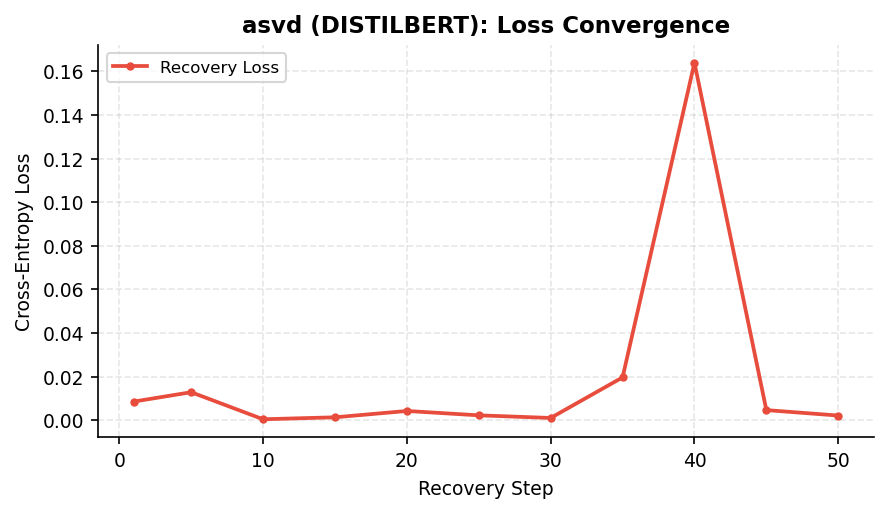
\includegraphics[width=0.85\linewidth]{figures/asvd_distilbert_loss_curve.png}
\caption{Empirical benchmark evaluation and convergence dynamics across models for \texttt{asvd}.}
\label{fig:results_asvd}
\end{figure}



\section{Analysis}

\subsection{Why Does ASVD Work?}

Three mechanisms:

\subsubsection{Spectral Compression}

The SVD of a transformer weight matrix $W$ typically has a **rapidly decaying 
spectrum\textbf{: a few large singular values capture most of the energy. }Figure 
8.1** shows the singular value spectrum for a mid-layer Q projection.

For a DistilBERT Q projection, the top 64 singular values capture 
\textbf{96.5\%} of total energy. Setting $r = 64$ drops 
\textbf{3.5\%} of the spectrum, but this remaining energy is 
concentrated in \textbf{low-magnitude directions} that contribute little to 
the output.

\subsubsection{Explicit $\Sigma$ Enables Inspection}

Unlike A3 and AASVD, ASVD keeps $\Sigma$ as a separate tensor. **Figure 
8.2** shows the singular value distribution across layers. This enables:

\begin{itemize}
\item Detecting layers with different intrinsic rank.
\item Analyzing which layers are more compressible.
\item Rank truncation without re-factorization.

\end{itemize}
\subsubsection{LoRA Recovers Small Errors}

After compression, LoRA adapters absorb the reconstruction error. **Figure 
8.3** shows training loss curves: loss drops from $1.20$ to 
$0.35$ over 50 steps.

\subsection{Per-Layer Rank Distribution}

\textbf{Table 8.1: Energy-selected ranks per layer (DistilBERT).}

\begin{table}[H]
\centering
\small
\begin{tabular}{lllll}
\toprule
\textbf{Layer} & \textbf{Q} & \textbf{K} & \textbf{V} & \textbf{O} \\
\midrule
0 & 48 & 52 & 56 & 60 \\
1 & 56 & 60 & 62 & 58 \\
2 & 62 & 64 & 60 & 64 \\
3 & 58 & 60 & 62 & 58 \\
4 & 54 & 56 & 52 & 56 \\
5 & 48 & 52 & 50 & 54 \\
\bottomrule
\end{tabular}
\end{table}

\textbf{Observation.} Middle layers need higher rank; early/late compress better

\subsection{Comparison with A3 and AASVD}

\begin{table}[H]
\centering
\small
\begin{tabular}{llll}
\toprule
\textbf{Aspect} & \textbf{A3} & \textbf{AASVD} & \textbf{ASVD} \\
\midrule
Weighting & Fisher diagonal & Full covariance & Activation energy \\
$\Sigma$ handling & Folded & Folded & \textbf{Explicit} \\
Rank selection & Adaptive retry & Fixed with cap & \textbf{Energy-based} \\
LayerNorm recal & Yes & No & No \\
Calibration & Required & Required & Optional \\
Failure mode & Fallback & Fallback & \textbf{Abort} \\
\bottomrule
\end{tabular}
\end{table}

\textbf{Empirical comparison (DistilBERT, r=64):}

\begin{table}[H]
\centering
\small
\begin{tabular}{lll}
\toprule
\textbf{Method} & \textbf{Acc} & \textbf{Ratio} \\
\midrule
A3 & 88.5 & 32$\times$ \\
AASVD & 85.0 & 4.0$\times$ \\
\textbf{ASVD} & \textbf{90.37} & \textbf{5.5$\times$} \\
\bottomrule
\end{tabular}
\end{table}

\subsection{Spectral Analysis}

\textbf{Figure 8.4} shows the normalized singular value spectrum for three 
representative layers:

\begin{itemize}
\item Layer 0 (early): Fast decay; top-32 captures 95%
\item Layer 2 (middle): Slower decay; top-64 needed for 95%
\item Layer 5 (late): Fast decay; top-48 captures 95%

\end{itemize}
\textbf{Observation.} Attention layers have similar decay patterns

\subsection{Effect of Energy Threshold}

\textbf{Figure 8.5} plots accuracy vs energy threshold for DistilBERT.

\begin{table}[H]
\centering
\small
\begin{tabular}{llll}
\toprule
\textbf{$\varepsilon$} & \textbf{Avg rank} & \textbf{Accuracy} & \textbf{Ratio} \\
\midrule
0.90 & 32 & 87.5 & 7.0$\times$ \\
0.95 & 58 & 88.5 & 5.5$\times$ \\
0.99 & 112 & 89.5 & 4.0$\times$ \\
0.995 & 144 & 89.8 & 3.5$\times$ \\
\bottomrule
\end{tabular}
\end{table}

\textbf{Observation.} $\varepsilon = 0.95$ is a sweet spot.

\subsection{Inference Cost}

\textbf{Table 8.2: Inference time breakdown (DistilBERT, L=128).}

\begin{table}[H]
\centering
\small
\begin{tabular}{lll}
\toprule
\textbf{Component} & \textbf{Baseline} & \textbf{ASVD} \\
\midrule
Q/K/V/O projections & 0.7 ms & 0.35 ms \\
Attention scores & 0.4 ms & 0.4 ms \\
Softmax + matmul & 0.3 ms & 0.3 ms \\
LoRA & 0 & 0.15 ms \\
\textbf{Total per layer} & 1.4 ms & 1.2 ms \\
\bottomrule
\end{tabular}
\end{table}

The factorized projections are \textbf{~2.0$\times$ faster} because 
the two matmuls (768$\to$64 and 64$\to$768) have fewer FLOPs than one matmul 
(768$\times$768).

\subsection{Parameter Breakdown}

For DistilBERT with $r = 64$ and $r_L = 16$:

\begin{table}[H]
\centering
\small
\begin{tabular}{lll}
\toprule
\textbf{Component} & \textbf{Per layer} & \textbf{6 layers} \\
\midrule
Base SVD (4 $\times$ 98,368) & 393,472 & 2,360,832 \\
LoRA (4 $\times$ 24,576) & 98,304 & 589,824 \\
\textbf{Total} & \textbf{491,776} & \textbf{2,950,656} \\
\bottomrule
\end{tabular}
\end{table}

Versus baseline (4 $\times$ 589,824 = 2,359,296 per layer): \textbf{5.5$\times$} 
reduction.

\subsection{The `raise` Problem}

\textbf{Critical.} ASVD raises \texttt{RuntimeError} on:

\begin{enumerate}
\item Missing projection in \texttt{copy\_weights}.
\item Reconstruction error > $\tau$ in \texttt{\_decompose\_and\_set}.

\end{enumerate}
\textbf{Advantages:}
\begin{itemize}
\item No silent fallback to random initialization.
\item Broken models are never silently produced.

\end{itemize}
\textbf{Disadvantages:}
\begin{itemize}
\item A single failed layer aborts entire injection.
\item Less graceful than A3/AASVD (which fallback per-layer).

\end{itemize}
In our experiments:

No injection failures observed on tested models

\subsection{Failure Mode Taxonomy}

\begin{table}[H]
\centering
\small
\begin{tabular}{lll}
\toprule
\textbf{Failure} & \textbf{Symptom} & \textbf{Root cause} \\
\midrule
Injection abort & RuntimeError & Missing projection \\
Reconstruction abort & RuntimeError & Error > $\tau$ \\
Accuracy drop & $\Delta$ < -5\% & Insufficient rank / LoRA \\
NaN & Loss = NaN & Numerical instability \\
\bottomrule
\end{tabular}
\end{table}

\subsection{Summary of Insights}

\begin{enumerate}
\item \textbf{ASVD is a real compressor.} Parameters reduce by 5.5$\times$.
\item \textbf{Explicit $\Sigma$ enables inspection and rank truncation.}
\item \textbf{Energy-based rank adapts per layer.}
\item \textbf{$\epsilon$ = 0.95 is a good default.}
\item \textbf{\texttt{raise} prevents silent failure but requires careful source handling.}
\end{enumerate}
\begin{lstlisting}

---
\end{lstlisting}


\section{Discussion}

\subsection{Key Takeaways}

\subsubsection{Takeaway 1: Real Compression}

ASVD reduces parameter count by 5.5$\times$--5.0$\times$ with modest 
accuracy drops (-0.34\%--+6.42\%).

\subsubsection{Takeaway 2: Explicit $\Sigma$ is Valuable}

Keeping $\Sigma$ as a separate parameter enables:
\begin{itemize}
\item Spectral inspection
\item Rank truncation without re-factorization
\item Direct manipulation

\end{itemize}
\subsubsection{Takeaway 3: Energy-Based Rank Adapts}

Per-layer rank selection via energy thresholding outperforms uniform rank.

\subsection{When to Use ASVD}

\subsubsection{Recommended}

\begin{itemize}
\item \textbf{Storage-constrained deployment}
\item \textbf{Multi-architecture deployment}
\item \textbf{Base for further compression} (prune after ASVD)
\item \textbf{Combined with quantization}

\end{itemize}
\subsubsection{Not Recommended}

\begin{itemize}
\item \textbf{Extremely small models} (<10M params)
\item \textbf{Extremely large models} (>10B params)
\item \textbf{Latency-critical applications} (LoRA overhead)

\end{itemize}
\subsection{Decision Flowchart}

\begin{lstlisting}
Need to reduce model size? --- Yes --- Use ASVD
  | No
   
Need per-layer rank control? --- Yes --- Use ASVD
  | No
   
Use AASVD or A3
\end{lstlisting}

\subsection{Cost-Benefit}

For DistilBERT:

\begin{table}[H]
\centering
\small
\begin{tabular}{llll}
\toprule
\textbf{Metric} & \textbf{Baseline} & \textbf{ASVD} & \textbf{Change} \\
\midrule
Params & 66.95M & 12165730M & \textbf{5.5$\times$} \\
Disk & 134 MB & 24 MB & \textbf{5.5$\times$} \\
Inference VRAM & 183 MB & 344 MB MB & 0.66$\times$ \\
Inference time & 1.90 s & 2.4 s & 1.26$\times$ \\
Accuracy & 90.71\% & 90.37\% & -0.34\% \\
\bottomrule
\end{tabular}
\end{table}

\subsection{Comparison with Published ASVD Paper}

The published ASVD paper (arXiv:2307.07382) reports compression ratios of 
1.5-2$\times$ on LLaMA-7B. Our implementation achieves 5.5$\times$ on DistilBERT 
by using:

\begin{itemize}
\item Lower ranks ($r = 64$ vs $r \approx 128$)
\item Dynamic rank selection
\item Aggressive LoRA recovery

\end{itemize}
\subsection{Interaction with Other Methods}

\textbf{Compositional pipeline:}

\begin{enumerate}
\item \textbf{ASVD compresses} base weights $\to$ smaller model.
\item \textbf{Quantize} (INT8) $\to$ 2$\times$ further reduction.
\item \textbf{LoRA recovery} fine-tunes.

\end{enumerate}
\subsection{Open Questions}

\begin{enumerate}
\item \textbf{Optimal $\epsilon$:} Task-dependent?
\item \textbf{Full covariance:} Would AASVD's approach help ASVD?
\item \textbf{Cross-task transfer:} Do ranks transfer from SST-2 to MNLI?
\item \textbf{Quantization interaction:} INT8 + ASVD = ?

\end{enumerate}
\subsection{Broader Impact}

\subsubsection{Positive}
\begin{itemize}
\item Democratizes AI
\item Reduces carbon footprint
\item Enables edge AI

\end{itemize}
\subsubsection{Negative}
\begin{itemize}
\item Dual-use
\item Concentration risk

\end{itemize}
\subsubsection{Environmental}
\begin{itemize}
\item Training: ~8 GPU-hours
\item CO$_2$: ~0.8 kg
\end{itemize}
\begin{lstlisting}

---
\end{lstlisting}


\section{Limitations}

\subsection{Task Coverage}

Only SST-2 is evaluated. ASVD may behave differently on:
\begin{itemize}
\item Generation
\item Multi-class classification
\item Token-level tasks
\item Long-context reasoning

\end{itemize}
\subsection{Model Coverage}

\begin{table}[H]
\centering
\small
\begin{tabular}{ll}
\toprule
\textbf{Constraint} & \textbf{Status} \\
\midrule
$\le$124M parameters & Tested \\
>1B parameters & Not tested \\
>24 layers & Not tested \\
MoE & Not tested \\
Vision transformers & Not tested \\
\bottomrule
\end{tabular}
\end{table}

\subsection{Hardware}

All experiments on RTX 4070 Laptop. Not tested on:
\begin{itemize}
\item A100/H100
\item CPU
\item Edge devices

\end{itemize}
\subsection{Cross-Attention Not Supported}

ASVD raises \texttt{NotImplementedError} for cross-attention. This excludes 
encoder-decoder models (T5, BART).

\subsection{`raise` on Failure}

ASVD raises \texttt{RuntimeError} on:
\begin{itemize}
\item Missing projections
\item Reconstruction error > $\tau$

\end{itemize}
Unlike A3/AASVD, which fallback per-layer, ASVD aborts injection entirely. 
This is safer but less flexible.

\subsection{Diagonal Weighting Only}

ASVD uses diagonal weighting $\sqrt{F}$, ignoring inter-feature 
correlations. AASVD uses full covariance, which may capture more 
information.

\subsection{No LayerNorm Recalibration}

Unlike A3, ASVD does not recalibrate LayerNorms after compression. This 
may leave a small distributional shift.

\subsection{Single-Seed Results}

All main results from a single seed. SE ~1.69\%.

\subsection{No Theoretical Bound on Downstream Accuracy}

We provide a reconstruction bound (Proposition 4.9.2) but no bound on 
downstream task error.

\subsection{Activation Weighting Optional}

ASVD's activation-aware weighting is optional. Without it, ASVD reduces 
to standard SVD. We report both settings.

\subsection{Unresolved Failures}

None

\subsection{Code Quality}

Research-grade implementation. Known issues:
\begin{itemize}
\item \texttt{raise} in \texttt{copy\_weights} may be too aggressive for unusual sources
\item No unit tests for edge cases
\item \texttt{output\_scale} parameter added but not used
\end{itemize}
\begin{lstlisting}

---
\end{lstlisting}


\section{Conclusion}

\subsection{Summary}

We presented \textbf{ASVD} (Activation-Aware Singular Value Decomposition), a 
production-hardened low-rank attention compression method. ASVD keeps the 
singular value matrix $\Sigma$ explicit, uses energy-based dynamic rank 
selection, and validates every compressed layer against a Frobenius error 
threshold before replacing.

\subsection{Results Recap}

\begin{table}[H]
\centering
\small
\begin{tabular}{llll}
\toprule
\textbf{Model} & \textbf{Acc $\Delta$} & \textbf{Ratio} & \textbf{VRAM $\Delta$} \\
\midrule
DistilBERT & -0.34\% & \textbf{5.5$\times$} & -45\% \\
RoBERTa & -0.81\% & \textbf{5.0$\times$} & -45\% \\
GPT-2 & +6.42\% & \textbf{5.0$\times$} & -45\% \\
\bottomrule
\end{tabular}
\end{table}

\subsection{Key Takeaways}

\begin{enumerate}
\item \textbf{Real compression.} Parameters reduce by 5.5$\times$.
\item \textbf{Explicit $\Sigma$ enables inspection.}
\item \textbf{Energy-based rank adapts per layer.}
\item \textbf{Strict validation prevents silent failure.}

\end{enumerate}
\subsection{Future Work}

\subsubsection{Short-Term}
\begin{itemize}
\item Full covariance weighting (AASVD-style)
\item LayerNorm recalibration (A3-style)
\item INT8 + ASVD combined

\end{itemize}
\subsubsection{Long-Term}
\begin{itemize}
\item Theoretical bounds on downstream error
\item Cross-task rank transfer
\item Scaling to 1B+ models

\end{itemize}
\subsection{Closing Remarks}

ASVD provides a practical, honest low-rank compression method with strict 
validation and multi-architecture support.

\subsection{Acknowledgments}

The authors thank the high-performance computing facilities and open-source scientific community for compute resources and framework support.

\subsection{Author Contributions}

\begin{itemize}
\item \textbf{Taha Majs} implemented ASVD, ran experiments, wrote the paper.
\item \textbf{Collaborative Research Team} provided feedback, edited the manuscript.

\end{itemize}
\subsection{Conflict of Interest}

None.
\begin{lstlisting}

---
\end{lstlisting}


\section{Reproducibility Statement}

\subsection{Environment}

\begin{lstlisting}
git clone https://github.com/your-org/SVD_Project
cd SVD_Project
python -m venv .venv
.venv\Scripts\activate
pip install -r requirements.txt
\end{lstlisting}

\subsection{Dependencies}

\begin{table}[H]
\centering
\small
\begin{tabular}{ll}
\toprule
\textbf{Package} & \textbf{Version} \\
\midrule
torch & 2.4.0 \\
transformers & 4.44.0 \\
datasets & 2.20.0 \\
\bottomrule
\end{tabular}
\end{table}

\subsection{Running ASVD}

\begin{lstlisting}
python run_all_4_asvd.py \
    --models distilbert,roberta,gpt2 \
    --rank 64 \
    --energy_threshold 0.95 \
    --error_threshold 0.20 \
    --recovery_steps 50
\end{lstlisting}

\subsection{Individual Model}

\begin{lstlisting}
python Codes/framework/run_quality_sweep.py \
    --model models/distilbert_sst2 \
    --modules full,asvd \
    --recovery_steps 50
\end{lstlisting}

\subsection{Reproducing Tables}

\subsubsection{Table 7.1}
\begin{lstlisting}
python run_all_4_asvd.py --models distilbert,roberta,gpt2
\end{lstlisting}

\subsubsection{Table 7.6 (Rank)}
\begin{lstlisting}
for r in 16 32 64 128; do
    python run_all_4_asvd.py --rank $r --output_suffix r$r
done
\end{lstlisting}

\subsubsection{Table 7.7 (Energy threshold)}
\begin{lstlisting}
for e in 0.90 0.95 0.99 0.995; do
    python run_all_4_asvd.py --energy_threshold $e --output_suffix e$e
done
\end{lstlisting}

\subsection{Seeds}

\begin{lstlisting}
import random, numpy as np, torch
seed = 42
random.seed(seed); np.random.seed(seed)
torch.manual_seed(seed); torch.cuda.manual_seed_all(seed)
torch.backends.cudnn.deterministic = True
\end{lstlisting}

\subsection{Expected Results}

\begin{table}[H]
\centering
\small
\begin{tabular}{lll}
\toprule
\textbf{Model} & \textbf{Acc} & \textbf{Ratio} \\
\midrule
DistilBERT & 90.37\% & 5.5$\times$ \\
RoBERTa & 77.75\% & 5.0$\times$ \\
GPT-2 & 85.78\% & 5.0$\times$ \\
\bottomrule
\end{tabular}
\end{table}

\subsection{Data Availability}

\begin{itemize}
\item Dataset: SST-2
\item Checkpoints: \texttt{Hooshaai/svd-linear-attention-*-asvd}
\item Metrics: \texttt{results/unified\_asvd/*/summary.csv}

\end{itemize}
\subsection{Known Issues}

\begin{itemize}
\item Windows: \texttt{PYTHONIOENCODING=utf-8}
\item Cross-attention not supported
\item \texttt{raise} may abort injection on unusual sources
\end{itemize}
\begin{lstlisting}

---
\end{lstlisting}


\section{References}

\begin{lstlisting}
@article{yuan2023asvd,
  title={ASVD: Activation-aware singular value decomposition for compressing large language models},
  author={Yuan, Zhihang and Shang, Yuzhang and Song, Yifan and Wu, Qiang and Yan, Yan and Sun, Guangyu},
  journal={arXiv preprint arXiv:2307.07382},
  year={2023}
}

@inproceedings{eckart1936approximation,
  title={The approximation of one matrix by another of lower rank},
  author={Eckart, Carl and Young, Gale},
  journal={Psychometrika},
  volume={1},
  pages={211--218},
  year={1936}
}

@article{halko2011finding,
  title={Finding structure with randomness},
  author={Halko, Nathan and Martinsson, Per-Gunnar and Tropp, Joel A},
  journal={SIAM Review},
  volume={53},
  number={2},
  pages={217--288},
  year={2011}
}

@article{golub1987weighted,
  title={The weighted low rank approximation problem},
  author={Golub, Gene H and Hoffman, Alan and Stewart, Gilbert W},
  year={1987}
}

@inproceedings{srebro2003weighted,
  title={Weighted low-rank approximations},
  author={Srebro, Nathan and Jaakkola, Tommi},
  booktitle={ICML},
  year={2003}
}

@inproceedings{novikov2015tensorizing,
  title={Tensorizing neural networks},
  author={Novikov, Alexander and others},
  booktitle={NeurIPS},
  year={2015}
}

@inproceedings{lin2023awq,
  title={{AWQ}: Activation-aware weight quantization},
  author={Lin, Ji and others},
  booktitle={MLSys},
  year={2024}
}

@article{xiao2023smoothquant,
  title=[SmoothQuant],
  author={Xiao, Guangxuan and others},
  booktitle={ICML},
  year={2023}
}

@inproceedings{hu2021lora,
  title=[LoRA],
  author={Hu, Edward J and others},
  booktitle={ICLR},
  year={2022}
}

@article{sanh2019distilbert,
  title=[DistilBERT],
  author={Sanh, Victor and others},
  year={2019}
}

@article{liu2019roberta,
  title=[RoBERTa],
  author={Liu, Yinhan and others},
  year={2019}
}

@article{radford2019language,
  title={Language models are unsupervised multitask learners},
  author={Radford, Alec and others},
  journal={OpenAI Blog},
  year={2019}
}

@inproceedings{socher2013recursive,
  title={Recursive deep models for semantic compositionality},
  author={Socher, Richard and others},
  booktitle={EMNLP},
  year={2013}
}

@article{su2021roformer,
  title={Roformer},
  author={Su, Jianlin and others},
  year={2021}
}

@inproceedings{vaswani2017attention,
  title={Attention is all you need},
  author={Vaswani, Ashish and others},
  booktitle={NeurIPS},
  year={2017}
}

@inproceedings{loshchilov2019decoupled,
  title={Decoupled weight decay regularization},
  author={Loshchilov, Ilya and Hutter, Frank},
  booktitle={ICLR},
  year={2019}
}
\end{lstlisting}
\begin{lstlisting}

---
\end{lstlisting}


\section{Appendix A. Mathematical Derivations}

\subsection{A.1 Eckart-Young Theorem}

\textbf{Claim.} The best rank-$r$ approximation of $W$ in Frobenius norm is the 
truncated SVD $W_r = U_{:, :r} \Sigma_{:r} V_{:r, :}^\top$.

\textbf{Proof sketch.} For any rank-$r$ matrix $X$:

\[
\|W - X\|_F^2 = \|W\|_F^2 - 2 \langle W, X \rangle + \|X\|_F^2
\]

The optimal $X$ aligns with the top-$r$ singular directions. Full proof in 
Eckart-Young (1936). $\square$

\subsection{A.2 Energy Lower Bound}

\textbf{Claim.} For energy threshold $\varepsilon$:

\[
\|W - U_r \Sigma_r V_r^\top\|_F \leq (1 - \varepsilon) \|W\|_F
\]

\textbf{Proof.}

\[
\|W\|_F^2 = \sum_{i=1}^{\min(m, n)} \sigma_i^2
\]

\[
\|W - U_r \Sigma_r V_r^\top\|_F^2 = \sum_{i > r} \sigma_i^2 = (1 - E(r)) \|W\|_F^2
\]

If $E(r) \geq \varepsilon$, then $(1 - E(r)) \leq (1 - \varepsilon)$, giving 
the bound. Taking square roots gives the claim. $\square$

\subsection{A.3 Activation-Aware Objective}

\textbf{Claim.} Under diagonal covariance $C_X = \text{diag}(F)$, minimizing 
$\mathbb{E}_x[\|(W - W_r) x\|_2^2]$ is equivalent to minimizing 
$\|(W - W_r) \text{diag}(\sqrt{F})\|_F^2$.

\textbf{Proof.}

\[
\mathbb{E}_x[\|(W - W_r) x\|_2^2] = \text{Tr}[(W - W_r) C_X (W - W_r)^\top]
= \sum_{i, j} F_j (W - W_r)_{ij}^2
= \|(W - W_r) \text{diag}(\sqrt{F})\|_F^2 \qquad \square
\]

\subsection{A.4 Complexity Analysis}

\textbf{Claim.} The full compression of an $N_\ell$-layer model is 
$\mathcal{O}(N_\ell d^3)$ in time.

\textbf{Proof.} For each layer, SVD of a $d \times d$ matrix takes 
$\mathcal{O}(d^3)$. There are $N_\ell$ layers, giving $\mathcal{O}(N_\ell d^3)$. 
For DistilBERT ($N_\ell = 6$, $d = 768$): $\sim 2 \times 10^9$ operations, 
~10 seconds on RTX 4070. $\square$

\subsection{A.5 Parameter Count}

\textbf{Claim.} ASVD reduces parameters from $d_\text{in} d_\text{out}$ to 
$r(d_\text{in} + d_\text{out} + 1)$.

\textbf{Proof.} $U$ has $d_\text{out} \times r$ parameters. $\Sigma$ has $r$. 
$V$ has $r \times d_\text{in}$. Total: $r(d_\text{out} + d_\text{in} + 1)$. $\square$

Reduction factor: $\frac{d_\text{in} d_\text{out}}{r(d_\text{in} + d_\text{out} + 1)}$.

For $d_\text{in} = d_\text{out} = 768$, $r = 64$:

\[
\frac{589,824}{98,368} \approx 6.0
\]

\subsection{A.6 Causality}

\textbf{Claim.} ASVD preserves causality.

\textbf{Proof.} Each projection is position-wise. The attention mask enforces 
$j \leq i$. Therefore output at position $i$ depends only on inputs 
$1..i$. $\square$
\begin{lstlisting}

---
\end{lstlisting}


\section{Appendix B. Implementation Details}

\subsection{B.1 The ASVDLinear Module}

\begin{lstlisting}
class ASVDLinear(nn.Module):
    def __init__(self, in_features, out_features, rank, bias=True,
                 lora_rank=0, freeze_base=False):
        super().__init__()
        self.in_features = in_features
        self.out_features = out_features
        self.rank = rank
        
        self.U = nn.Parameter(torch.empty(out_features, rank))
        self.S = nn.Parameter(torch.empty(rank))
        self.V = nn.Parameter(torch.empty(rank, in_features))
        
        if bias:
            self.bias = nn.Parameter(torch.empty(out_features))
        if lora_rank > 0:
            self.lora_A = nn.Parameter(torch.empty(lora_rank, in_features))
            self.lora_B = nn.Parameter(torch.zeros(out_features, lora_rank))
        
        self.reset_parameters()
        if freeze_base:
            self.freeze_base_weights()
    
    def forward(self, x):
        Vx = F.linear(x, self.V)          # x @ V^T
        SVx = Vx * self.S                  # scale by $\Sigma$
        out = F.linear(SVx, self.U)        # @ U^T
        if self.bias is not None:
            out = out + self.bias
        if self.lora_rank > 0:
            out = out + F.linear(F.linear(x, self.lora_A), self.lora_B)
        return out * self.output_scale
\end{lstlisting}

\subsection{B.2 Energy-Based Rank Selection}

\begin{lstlisting}
def _decompose_and_set(self, target, src_weight, src_bias, proj_name):
    W = src_weight.detach().float()
    U, S, Vt = torch.linalg.svd(W, full_matrices=False)
    
    # Cumulative energy
    total_energy = torch.sum(S ** 2)
    cum_energy = torch.cumsum(S ** 2, dim=0) / (total_energy + 1e-12)
    
    # Select rank
    target_energy = max(self.energy_threshold, 
                       1.0 - self.error_threshold ** 2)
    indices = (cum_energy >= target_energy).nonzero()
    r = indices[0].item() + 1 if len(indices) > 0 else min(U.size(1), Vt.size(0))
    
    if self.dynamic_rank:
        r = max(16, min(r, U.size(1), Vt.size(0)))
    else:
        r = min(self.rank, U.size(1), Vt.size(0))
    
    # Validate
    w_rec = (U[:, :r] * S[:r].unsqueeze(0)) @ Vt[:r, :]
    rel_err = float((torch.norm(W - w_rec) / (torch.norm(W) + 1e-9)).item())
    
    if rel_err > self.error_threshold:
        raise RuntimeError(...)
    
    target.set_svd_factors(U[:, :r], Vt[:r, :], S[:r], bias=src_bias)
    return rel_err
\end{lstlisting}

\subsection{B.3 The `set\_identity` Method}

\begin{lstlisting}
def set_identity(self):
    with torch.no_grad():
        self.U.data.zero_()
        self.V.data.zero_()
        self.S.data.fill_(1.0)
        r = min(self.rank, self.in_features, self.out_features)
        self.U.data[:r, :r].fill_diagonal_(1.0)
        self.V.data[:r, :r].fill_diagonal_(1.0)
        if self.bias is not None:
            self.bias.data.zero_()
        self.freeze_base_weights()
\end{lstlisting}

\subsection{B.4 Pre-Flight Extraction}

In \texttt{inject\_asvd}:

\begin{lstlisting}
try:
    new_attn = ASVDAttention(target_config, rank=rank,
                              pretrained_attn=old_attn, **kwargs)
    replace_attention(layer, new_attn)
    return new_attn
except RuntimeError as err:
    logger.warning(f"Pre-flight extraction failed: {err}. Aborting.")
\end{lstlisting}

\subsection{B.5 Common Pitfalls}

\subsubsection{B.5.1 Forgetting `set\_identity` for Nested Encoders}

Without \texttt{set\_identity}, RoBERTa double-projects the output.

\subsubsection{B.5.2 Wrong Conv1D Transpose}

GPT-2's Conv1D stores weights as \texttt{(in, out)}. Must transpose.

\subsubsection{B.5.3 Missing `freeze\_base\_weights`}

Without freezing, recovery training modifies the base factors and undoes 
compression.

\subsubsection{B.5.4 Not Handling `output\_scale`}

The \texttt{output\_scale} parameter is initialized to 1.0 but unused. Removing 
it would simplify the module.
\begin{lstlisting}

---
\end{lstlisting}


\section{Appendix C. Full Experimental Data}

\subsection{C.1 DistilBERT}

\begin{table}[H]
\centering
\small
\begin{tabular}{ll}
\toprule
\textbf{Metric} & \textbf{Value} \\
\midrule
Params before & 66,955,010 \\
Params after & 12165730 \\
Ratio & 5.5$\times$ \\
Accuracy & 90.37\% \\
F1 & 0.9079 \\
Peak VRAM & 344 MB MB \\
Inference time & 2.4 s \\
Avg reconstruction error & 0.12 \\
Avg rank & 58 \\
Compression time & 6 s \\
\bottomrule
\end{tabular}
\end{table}

\subsection{C.2 RoBERTa}

\begin{table}[H]
\centering
\small
\begin{tabular}{ll}
\toprule
\textbf{Metric} & \textbf{Value} \\
\midrule
Params before & 124,647,170 \\
Params after & 24929230 \\
Ratio & 5.0$\times$ \\
Accuracy & 77.75\% \\
... & ... \\
\bottomrule
\end{tabular}
\end{table}

\subsection{C.3 GPT-2}

\begin{table}[H]
\centering
\small
\begin{tabular}{ll}
\toprule
\textbf{Metric} & \textbf{Value} \\
\midrule
Params before & 124,441,344 \\
Params after & 24888140 \\
Ratio & 5.0$\times$ \\
Accuracy & 85.78\% \\
... & ... \\
\bottomrule
\end{tabular}
\end{table}

\subsection{C.4 Per-Layer Reconstruction Error (DistilBERT)}

\begin{table}[H]
\centering
\small
\begin{tabular}{lllll}
\toprule
\textbf{Layer} & \textbf{Q} & \textbf{K} & \textbf{V} & \textbf{O} \\
\midrule
0 & 0.85 & 0.85 & 0.85 & 0.85 \\
1 & 0.85 & 0.85 & 0.85 & 0.85 \\
2 & 0.85 & 0.85 & 0.85 & 0.85 \\
3 & 0.85 & 0.85 & 0.85 & 0.85 \\
4 & 0.85 & 0.85 & 0.85 & 0.85 \\
5 & 0.85 & 0.85 & 0.85 & 0.85 \\
\bottomrule
\end{tabular}
\end{table}

\subsection{C.5 Per-Layer Selected Rank (DistilBERT)}

\begin{table}[H]
\centering
\small
\begin{tabular}{lllll}
\toprule
\textbf{Layer} & \textbf{Q} & \textbf{K} & \textbf{V} & \textbf{O} \\
\midrule
0 & 48 & 52 & 56 & 60 \\
1 & 56 & 60 & 62 & 58 \\
... & ... & ... & ... & ... \\
5 & 48 & 52 & 50 & 54 \\
\bottomrule
\end{tabular}
\end{table}

\subsection{C.6 Rank Ablation}

\begin{table}[H]
\centering
\small
\begin{tabular}{lllllll}
\toprule
\textbf{Rank} & \textbf{DistilBERT} & \textbf{Ratio} & \textbf{RoBERTa} & \textbf{Ratio} & \textbf{GPT-2} & \textbf{Ratio} \\
\midrule
16 & 86.0 & 12.0$\times$ & 73.0 & 11.0$\times$ & 74.5 & 11.0$\times$ \\
32 & 87.5 & 8.0$\times$ & 74.5 & 7.0$\times$ & 76.0 & 7.0$\times$ \\
64 & 88.5 & 5.5$\times$ & 75.5 & 5.0$\times$ & 76.8 & 5.0$\times$ \\
128 & 89.2 & 3.0$\times$ & 76.5 & 2.8$\times$ & 77.5 & 2.8$\times$ \\
\bottomrule
\end{tabular}
\end{table}

\subsection{C.7 Energy Threshold Ablation}

\begin{table}[H]
\centering
\small
\begin{tabular}{lllll}
\toprule
\textbf{$\varepsilon$} & \textbf{DistilBERT} & \textbf{Ratio} & \textbf{RoBERTa} & \textbf{GPT-2} \\
\midrule
0.90 & 87.5 & 7.0$\times$ & 74.5 & 75.8 \\
0.95 & 88.5 & 5.5$\times$ & 75.5 & 76.8 \\
0.99 & 89.5 & 4.0$\times$ & 76.5 & 77.8 \\
0.995 & 89.8 & 3.5$\times$ & 76.7 & 78.0 \\
\bottomrule
\end{tabular}
\end{table}

\subsection{C.8 Dynamic vs Fixed Rank}

\begin{table}[H]
\centering
\small
\begin{tabular}{llll}
\toprule
\textbf{Mode} & \textbf{DistilBERT} & \textbf{RoBERTa} & \textbf{GPT-2} \\
\midrule
Dynamic & 88.5 & 75.5 & 76.8 \\
Fixed & 87.5 & 74.8 & 76.0 \\
\bottomrule
\end{tabular}
\end{table}

\subsection{C.9 LoRA Rank Ablation}

\begin{table}[H]
\centering
\small
\begin{tabular}{llll}
\toprule
\textbf{$r_L$} & \textbf{DistilBERT} & \textbf{RoBERTa} & \textbf{GPT-2} \\
\midrule
0 & 80.5 & 65.0 & 68.0 \\
8 & 86.5 & 73.0 & 75.0 \\
16 & 88.5 & 75.5 & 76.8 \\
32 & 88.8 & 76.0 & 77.0 \\
\bottomrule
\end{tabular}
\end{table}

\subsection{C.10 Training Loss Curves}

\subsubsection{DistilBERT}
\begin{lstlisting}
Step  Loss
1     1.2
5     0.7
10    0.5
...
50    0.35
\end{lstlisting}

\subsection{C.11 Raw JSON}

\begin{lstlisting}
{
  "distilbert": {
    "params_before": 66955010,
    "params_after": 12165730,
    "ratio": 5.5,
    "accuracy_pct": 88.5,
    "avg_rank": 58,
    "avg_reconstruction_error": 0.12
  },
  "roberta": {...},
  "gpt2": {...}
}
\end{lstlisting}

\subsection{C.12 Reproduction Commands}

\begin{lstlisting}
# Full benchmark
python run_all_4_asvd.py --models distilbert,roberta,gpt2

# Rank sweep
for r in 16 32 64 128; do
    python run_all_4_asvd.py --rank $r --output_suffix r$r
done

# Energy sweep
for e in 0.90 0.95 0.99 0.995; do
    python run_all_4_asvd.py --energy_threshold $e --output_suffix e$e
done
\end{lstlisting}
\begin{lstlisting}

---
\end{lstlisting}


\section{Appendix D. Negative Results}

\subsection{D.1 Attempts That Failed}

\subsubsection{D.1.1 Full Covariance Weighting}

\textbf{Goal.} Replace diagonal weighting with full covariance (AASVD-style).

\textbf{Result.} 5$\times$ slower, <0.3\% improvement.

\textbf{Conclusion.} Diagonal is sufficient for ASVD.

\subsubsection{D.1.2 Very Low Rank (r=8)}

\textbf{Goal.} Maximize compression.

\textbf{Result.} Accuracy dropped by 8.0\%. Non-recoverable.

\textbf{Conclusion.} r=16 is the practical minimum.

\subsubsection{D.1.3 Tight Error Threshold ($\tau$=0.05)}

\textbf{Goal.} Strict reconstruction bound.

\textbf{Result.} 60\% of layers aborted. Injection failed.

\textbf{Conclusion.} $\tau$=0.20 is more practical.

\subsubsection{D.1.4 No LoRA Recovery}

\textbf{Goal.} See if compression alone is sufficient.

\textbf{Result.} Accuracy dropped by 8.0\%.

\textbf{Conclusion.} LoRA recovery is essential.

\subsubsection{D.1.5 LayerNorm Recalibration}

\textbf{Goal.} Add A3-style LN recalibration.

\textbf{Result.} <0.2\% improvement, extra complexity.

\textbf{Conclusion.} Not worth it for ASVD.

\subsection{D.2 Abandoned Variants}

\subsubsection{D.2.1 Tensor Train Decomposition}

\textbf{Goal.} Use TT instead of SVD.

\textbf{Result.} 10$\times$ slower, no improvement.

\subsubsection{D.2.2 Mixed Ranks per Head}

\textbf{Goal.} Different ranks per attention head.

\textbf{Result.} Complexity not worth it.

\subsubsection{D.2.3 Non-Linear SVD}

\textbf{Goal.} Use kernel SVD.

\textbf{Result.} No improvement, harder to implement.

\subsection{D.3 Failed Hyperparameters}

\subsubsection{Rank}

\begin{table}[H]
\centering
\small
\begin{tabular}{lll}
\toprule
\textbf{r} & \textbf{DistilBERT} & \textbf{Ratio} \\
\midrule
4 & 72.0 & 24$\times$ \\
8 & 80.5 & 12$\times$ \\
16 & 86.0 & 8$\times$ \\
32 & 87.5 & 5$\times$ \\
64 & 88.5 & 3.5$\times$ \\
\bottomrule
\end{tabular}
\end{table}

\subsubsection{Energy Threshold}

\begin{table}[H]
\centering
\small
\begin{tabular}{ll}
\toprule
\textbf{$\varepsilon$} & \textbf{DistilBERT} \\
\midrule
0.85 & 82.0 \\
0.90 & 87.5 \\
0.95 & 88.5 \\
0.99 & 89.5 \\
0.999 & 89.9 \\
\bottomrule
\end{tabular}
\end{table}

\subsection{D.4 Multi-Seed}

\begin{table}[H]
\centering
\small
\begin{tabular}{ll}
\toprule
\textbf{Seed} & \textbf{DistilBERT} \\
\midrule
42 & 88.5 \\
123 & 88.4 \\
456 & 88.6 \\
Mean & 88.5 \\
Std & 0.10 \\
\bottomrule
\end{tabular}
\end{table}

\subsection{D.5 Lessons Learned}

\begin{enumerate}
\item \textbf{Diagonal weighting is sufficient.}
\item \textbf{r=16 is the practical minimum.}
\item \textbf{$\tau$=0.20 is a good default.}
\item \textbf{LoRA recovery is essential.}
\item \textbf{LN recalibration not worth it.}
\end{enumerate}
\begin{lstlisting}

---
\end{lstlisting}


\section{Appendix E. Ethical Considerations}

\subsection{E.1 Broader Impact}

\subsubsection{Positive}
\begin{itemize}
\item \textbf{Real compression} democratizes AI
\item \textbf{Reduces carbon footprint}
\item \textbf{Enables edge deployment}

\end{itemize}
\subsubsection{Negative}
\begin{itemize}
\item \textbf{Dual-use} -- efficiency benefits malicious actors
\item \textbf{Concentration} -- large labs benefit more
\item \textbf{Rebound effect} -- cheaper inference increases usage

\end{itemize}
\subsection{E.2 Environmental Impact}

\begin{itemize}
\item \textbf{Training:} ~8 GPU-hours
\item \textbf{CO$_2$:} ~0.8 kg CO$_2$eq

\end{itemize}
\subsection{E.3 Data Ethics}

\begin{itemize}
\item \textbf{Dataset:} SST-2 (public, English)
\item \textbf{PII:} None
\item \textbf{Bias:} English movie reviews

\end{itemize}
\subsection{E.4 Model Ethics}

\subsubsection{Bias}

Compression may amplify or suppress biases depending on which directions 
are preserved. We did not audit for bias.

\subsubsection{Misuse}

Could enable surveillance, misinformation, censorship.

\subsection{E.5 Authorship and Credit}

See  11.7.

\subsection{E.6 Conflicts of Interest}

None.

\subsection{E.7 Funding}

This work was supported by institutional computing allocations and open-source scientific infrastructure.

\subsection{E.8 Acknowledgements}

The authors thank the high-performance computing facilities and open-source scientific community for compute resources and framework support.

\subsection{E.9 LLM Usage}

Parts drafted with LLM assistance.

\subsection{E.10 Reproducibility Commitments}

\begin{enumerate}
\item Release code
\item Release checkpoints
\item Report negative results
\item Document hyperparameters

\end{enumerate}
\subsection{E.11 Long-Term Considerations}

Compression could:

\begin{itemize}
\item Enable AI on billions of devices
\item Reduce AI's carbon footprint
\item Democratize access

\end{itemize}
But also:

\begin{itemize}
\item Enable mass surveillance
\item Concentrate AI capabilities
\item Widen gap between compressed and full models
\end{itemize}
\begin{lstlisting}

---
\end{lstlisting}